\chapter{Design Methodology}
\label{ch:method}
This chapter briefly introduces a cell-based design methodology with an inherent ready-valid protocol. The methodology consists of a workflow and cell-based design library. To motivate the ease-of-use and applicability of the methodology, several complex examples are shown.

%\todo{
%- Read up on counterflow pipeline and see if there is an analogue.\\
%- Andy, do you think that your methodology only works for streaming based accelerators or for all kinds of logic? Did you try it with other types of logic as well?\\
%}





\section{Design Philosophy}
The methodology described is designed over a course of several years by Andrew K. Martin from the IBM Austin Research Lab. The initial ideas concerning this methodology originate from a paper published in 2001 called \textit{The Theory of Latency-Insensitive Design} \cite{delay-insensitive}. It describes the fundamentals of a correct-by-construction design methodology. This paper forms the basis of the ready-valid design methodology by Andrew K. Martin \cite{andy}.



\subsection{The Theory of Latency-Insensitive Design}
The paper \cite{delay-insensitive} presents a foundation of a correct-by-construction methodology which separates a system based on communication and computation. A system is defined as a set of synchronous computational processes that exchange data with one another over communication channels. An abstract protocol is used for communication whose main characteristic is to be insensitive to the latencies of the channels. The protocol works under the assumption that the computational processes are stallable and guarantees that computational processes behave correctly independently of the channel latencies. This enables changing the latency of a communication channel without affecting the functionality of the system, which is a useful property for hardware design.\\
Suppose a system is implemented, but due to wire delay timing constraints are not met. This theory guarantees that a relay station, or register, can be inserted in the communication channel without affecting the functionality. Therefore no costly redesigns are needed.\\
The idea of relay stations is borrowed from the pipelining concept and a relay station in function is similar to a register. This approach relaxes timing constraints during the early design phases when accurate measures of delay paths between computational processes are not yet available. If after physical implementation a mismatch exists between the timing constraint and the communication channel delays, they can easily be corrected by inserting the correct amount of relay stations. Since every computational process operates according to the latency-insensitive protocol, no changes are required in order to reflect the necessary changes in the communication channel latencies.



\subsection{Ready-Valid Design Methodology}
Typically, there are three types of flow control concepts a hardware designer can choose from.
\begin{itemize}
  \item{\textbf{Credit-Based} protocol manages credits between a start and end module. If no more credits are available, the logic in between is stalled.}
  \item{\textbf{Cycle-Based} protocol indicates after how many cycles a response will be received for sent data for example. A downside is that it is difficult to decide on what to do when no response is received, or more generally, what to do when the protocol breaks.}
  \item{\textbf{Ready-Valid-Based} protocol has a valid signal to indicate the validity of an output and a ready signal to indicate it is ready to receive a new input. Usually it is only used between large modules in a system.}
\end{itemize}

The ready-valid design methodology discussed here differs from the typical ready-valid protocol since it uses the paradigm all the way down to the lowest level of a system. This combined with the latency-insensitive design theory results in a methodology that consists of a library of cells that are analogous to the computational processes. These cells are interconnected using a ready-valid protocol, the communication channel, which makes it possible to stall at a cell granularity. This means that progress is made whenever possible.\\
The cell-based nature allows to easily understand a design by following the ready-valid protocol and associated data, if present. Due to a rich library of cells, writing a design mostly consists of connecting the cells and compiling the design. Since cells are correct-by-construction, errors only consist of typos, signal width mismatches, and other easily fixable errors. After that the ready-valid protocol is functionally correct. Only the associated data signals could not be functionally correct. This means that transformations on the data signal have been done incorrectly.



\subsection{Ready-Valid Communication Protocol}
In general, a cell within the ready-valid design methodology has a set of configuration parameters and a set of input and output signals, as shown in \autoref{fig:7-cell}. Examples of configuration parameters are the number of inputs or the signal width in bits of each data input. The input and output signals are named according to a predetermined scheme. The signals on the left of the generic cell are all called input signals, even though physically the ready signal is an output. Together they form the input interface and follow the naming convention of \texttt{i\_v} and \texttt{i\_r} for the valid and ready signal, respectively. The data signal, typically denoted by \texttt{i\_d}, is not obligatory and some cells only have ready and valid signals. According to the same naming convention, the output signals are called \texttt{o\_v}, \texttt{o\_d} and \texttt{o\_r} and together form the output interface.

\begin{figure}[H]
  \centering
  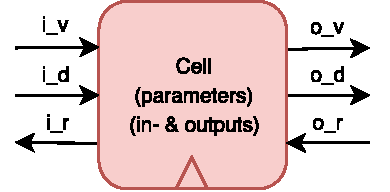
\includegraphics[width=0.50\textwidth]{7-cell.pdf}
  \caption{Input and output signals of a generic cell.}
  \label{fig:7-cell}
\end{figure}

The ready-valid protocol used by the cells on the communication channels between computational processes is a handshaking protocol. Progress is only made if both the input valid and ready signal are asserted for a cell in a given clock cycle. The communication channel is explicit and building a system mostly consists of connecting cells by a communication channel consisting of a ready and valid signal. In a system consisting of multiple cells, the naming convention dictates that a preceding cell is called \textit{upstream} and the successive cell is called \textit{downstream}.\\
In the ready-valid design methodology, a cell or computational processes can be combinatorial or sequential logic. Examples of each type will be shown in Section \ref{sec:cell-lib}. Independently of the type, a cell has at least two ready-valid signal pairs. One as input and one as output interface. In terms of physical input and output signals, a cell has two inputs, \texttt{i\_v} and \texttt{o\_r}, and two outputs, \texttt{i\_r} and \texttt{o\_v}.\\
Typically, when a cell comes out of a reset state, its input ready signal is asserted independently of any downstream cell ready signals it may receive at its output interface. The reason is that progress can be made by supplying the cell with a valid input to be serviced. The output valid signal is asserted when a valid input occurs and the cell is ready to service this valid input. In other words, the cell is not in a stalled state. If the cell is in a stalled state, the input ready signal will be de-asserted to indicate the upstream cells that a stall occurred. The concept of indicating to upstream cells that a cell is stalled is called \textit{applying back-pressure} in the ready-valid design methodology. An example of applying back-pressure could be that a cell requires data from multiple locations that do not arrive at the same time. Therefore, the cell has to be stalled until all data is available and back-pressure has to be applied to upstream cells. It is important to note that the input ready signal is only de-asserted if the cell is stalled, or if a downstream cell has stalled that induces a chain reaction of stalls. This is different from a typical ready-valid protocol where the ready signal is de-asserted after a transaction occurred (an example is AXI \cite{amba4}).



\subsection{Differences Compared to Asynchronous Design}
At first sight, the ready-valid design methodology may be interpreted as an asynchronous design methodology. However, there are several differences between the two. First of all, asynchronous design does not use a clock, while this methodology does. That means that the presentation of a ready or valid signal would be by changing the value of a signal, rather than by asserting it.\\
The ready-valid design methodology allows a ready or valid signal to be asserted in one cycle, and then de-assert in a subsequent cycle, even if the complimentary signal (valid or ready, respectively) was never asserted and no transaction took place. Similarly, the data corresponding with a valid signal is allowed to change on subsequent cycles, even though no corresponding ready signal was received and hence no data transfer took place. This would not work in an asynchronous framework and may have implications on design.\\
Finally, the \texttt{base\_aburp} and \texttt{base\_alatch} cells (discussed in Section \ref{sec:burp}) loose their meaning in an asynchronous framework. Although something analogous may be needed to maintain reasonable timing constraints between valid and data signals. 





\section{Workflow}
\label{sec:workflow}
Besides a supplied cell library, the ready-valid design methodology also comes with a workflow of several steps and special cells to speed up the workflow.
\begin{enumerate}
  \item{\textbf{Build the System} The first step is build the system with the provided cells, possibly accompanied by other logic. Relay stations should be placed between combinatorial cells and with experience proper locations are easily identified. These relay stations are analogous to configurable registers.}
  \item{\textbf{Functional Verification} After compiling the design from Step 1 and fixing compiler errors and warnings, the ready and valid signals should be verified first. Make sure they are always defined and only then verify the associated data signals. If more in-depth debugging is required, trace the valid and ready signals throughout the system and make sure cells apply back-pressure when needed, in order to not lose valid information.}
  \item{\textbf{Synthesis and Timing Constraints} After functional verification, the system should be synthesised to see if it meets the timing constraints. If the constraints are met, the next step can be started. If the constraints are not met, the register cells instantiated in Step 1 should simply be reconfigured accordingly or inserted multiple times to allow for multi-cycle communication channels; this step should be restarted. This process continues until the timing constraints are met everywhere in the design.}
  \item{\textbf{Physical Verification} After meeting the timing constraints, the system has to be verified again. When this step finishes successfully, it is possible to go back to Step 3 and tweak the design in order to improve metrics such as area or operating frequency.}
\end{enumerate}



\subsection{Tweaking Relay Stations}
The positioning of registers or relay stations depends on whether the system will be implemented on an ASIC or FPGA. For an FPGA, distribution of the wires is more difficult than driving them. FPGAs have buffers and repeaters everywhere to simplify this for the designer.\\
An ASIC does not have this luxury, thus the instinct of the designer concerning relay station positioning should be different. For ASICs, driving strength is more difficult. Positioning relay stations should take the combinatorial path of the function that is being implemented into account.



\subsection{Synthesis Helper Cells}
Systems or modules within a system typically have a large number of input and output signals, especially when data widths are large. When implementing a design on an FPGA, the provided tools try to connect each input or output signal of the system or module to a physical pin on the FPGA package. Depending on the size of the system or module and target device, there might not be enough physical pins for the tool to finish implementation. However, obtaining an estimate on metrics such as area and operating frequency is often desired, also for modules within the system.\\
In order to speedup synthesis and overcome the described problem, two helper cells are present in the cell library called \texttt{base\_input\_lat} and \texttt{base\_output\_lat}. These modules are parametrised shift registers. The \texttt{base\_input\_lat} cell is to be attached to one physical pin on the FPGA package and to all input signals of the system or module to be synthesised. Similarly but in opposite direction, the \texttt{base\_output\_lat} cell is used to connect multiple output signals to a single physical pin.





\section{Delay-Insensitive Cell Library}
\label{sec:cell-lib}
The cell library that is part of the ready-valid design methodology has been published on GitHub \cite{andy-lib} and is a work in progress. At the moment of writing, the version published on November 16, 2017 is used throughout this document.



\subsection{Diagram Legend and Naming Conventions}
Throughout this thesis, implementation diagrams and signal names follow a predefined scheme consisting of object shapes and colors and naming conventions to indicate various characteristics.



\subsubsection{Diagram Legend}
\label{sec:legend}
A cell is a submodule that is part of the design library. \autoref{fig:6-library-1} shows a combinatorial cell and \autoref{fig:6-library-2} a sequential cell. \autoref{fig:6-library-3} shows a (de)multiplexer cell, depending on the direction of the input and output signals.\\
Besides cells from the library, also logic that is not a cell can be included in a design called a submodule, shown in \autoref{fig:6-library-4}. \autoref{fig:6-library-5} shows a combinatorial arithmetic operation. A typical example is an addition to increment a counter. That could be implemented using a sequential cell. A common construct in this methodology is shown in \autoref{fig:6-library-6} and is called an act signal, often denoted by \texttt{*\_act}. It is a logical AND operation on a valid and ready signal, for example used as an enable signal.\\
To allow for hierarchy in diagrams, a collection of multiple cells and submodules can be replaced by a module. The module name always starts with a capital and is shown in \autoref{fig:6-library-7}. To show multiple identical instantiations of a cell or module, a generate construct is indicated by a green box. Multiple objects stacked behind each other and the number of instantiations is shown in the lower right corner, as shown in \autoref{fig:6-library-8}. The input and output signals are solid lines for the first instantiated object and dashed for any other objects stacked behind it.\\
Typically, only the downstream signals are shown in the diagrams and only rarely are upstream signals shown, such as ready signals. An act construct typically shows the ready signal until it is terminated.

\begin{figure}[h]
  \begin{subfigure}{.33\textwidth}
    \centering
    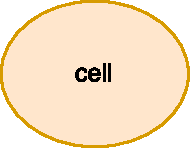
\includegraphics[width=0.60\linewidth]{6-library-1.pdf}
    \caption{Combinatorial cell.}
    \label{fig:6-library-1}
  \end{subfigure}%
  \begin{subfigure}{.33\textwidth}
    \centering
    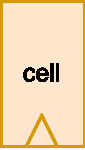
\includegraphics[width=0.25\linewidth]{6-library-2.pdf}
    \caption{Sequential cell.}
    \label{fig:6-library-2}
  \end{subfigure}%
  \begin{subfigure}{.33\textwidth}
    \centering
    
\includegraphics[width=0.15\linewidth]{6-library-3.pdf}
    \caption{(De)multiplexer cell.}
    \label{fig:6-library-3}
  \end{subfigure}\\[1ex]
  \begin{subfigure}{.33\textwidth}
    \centering
    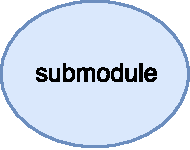
\includegraphics[width=0.60\linewidth]{6-library-4.pdf}
    \caption{Combinatorial submodule.}
    \label{fig:6-library-4}
  \end{subfigure}%
  \begin{subfigure}{.33\textwidth}
    \centering
    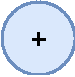
\includegraphics[width=0.25\linewidth]{6-library-5.pdf}
    \caption{Combinatorial arithmetic.}
    \label{fig:6-library-5}
  \end{subfigure}%
  \begin{subfigure}{.33\textwidth}
    \centering
    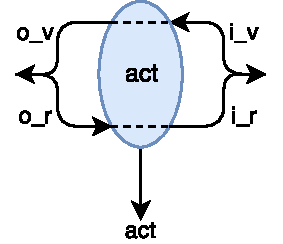
\includegraphics[width=0.80\linewidth]{6-library-6.pdf}
    \caption{Act signal.}
    \label{fig:6-library-6}
  \end{subfigure}\\[1ex]
  \begin{subfigure}{.5\textwidth}
    \centering
    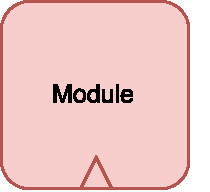
\includegraphics[width=0.40\linewidth]{6-library-7.pdf}
    \caption{Clocked module.}
    \label{fig:6-library-7}
  \end{subfigure}%
  \begin{subfigure}{0.5\textwidth}
    \centering
    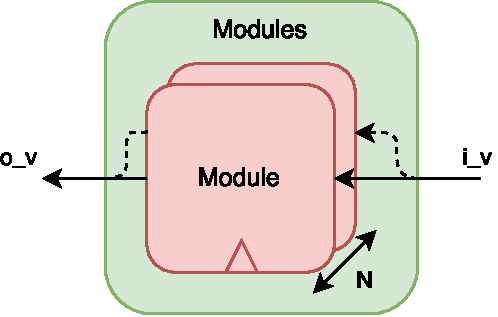
\includegraphics[width=0.80\linewidth]{6-library-8.pdf}
    \caption{Generate construct.}
    \label{fig:6-library-8}
  \end{subfigure}
  \caption{Implementation diagram conventions.}
  \label{fig:6-library}
\end{figure}

%\todo{
%- Fix vertical alignment.\\
%- Fix combinatorial arithmetic cutoff.\\
%}



\subsubsection{Naming Conventions}
Typically the input and output signals of any cell or module start with \texttt{i\_*} and \texttt{o\_*}, respectively. Internal signals of a cell or module also follow a naming convention, depending on the location of the signal with respect to the sequential elements and whether the signal has a special purpose, such as valid, ready, data, or act. Often the cell or module the valid signal originates from is included in the signal name. An example could be the output valid signal of the initial register cell: \texttt{s1\_reg\_v}. Another example could be a data signal after a counter cell operating after four pipeline stages from the input signals: \texttt{s4\_cntr\_d}. Listings shown later on provide more naming convention examples.\\
Cell or module instantiations follow a similar naming convention, indicating the pipeline stage the signal operates in, the cell or module name and indication if it is a combinatorial or sequential element. Typically combinatorial elements have no suffix while sequential elements have a \texttt{*\_reg} or \texttt{*\_lat} suffix, standing for register and latch, respectively. In the design methodology, a register is a sequential cell with a ready-valid pair as input and output. A latch is a sequential cell without ready-valid pairs.\\
Most cells have a prefix, either \texttt{a*} or \texttt{e*}. For historic reasons, the \texttt{a*} stands for \textit{asynchronous} and is used to mean that the cell has a ready-valid interface. The \texttt{e*} prefix means \textit{encoded} and typically refers to the select signal. Cells without this prefix typically have a decoded select signal.\\
Most of the cells are implemented as big-endian, but for certain cells the endianness matters. For example for multiplexers. For those cells a little-endian variant exists and is denoted by the suffix \texttt{*\_le}.





\subsection{Pass Gate Cell}
%\todo{
%- listing: fix white lines in dark background.\\
%- listing: center code \url{http://www.mrunix.de/forums/showthread.php?43153-lstinputlisting-zentriert}\\
%- listing: highlight Verilog function clog2 for example.\\
%- listing: highlight module instantiation.\\
%- listing: highlight bit signals "1'b1"\\
%}

A basic cell is the pass gate \texttt{agate} shown in \autoref{lst:gate}. Due to its straightforward behavior, it acts as an initial example of a cell from the library. The function of the cell is to grant access to a downstream ready-valid cell if a certain condition is met. The condition is supplied to the cell as the one bit input enable signal \texttt{en}. The cell has two additional input signals that are the input valid signal \texttt{i\_v} and output ready signal \texttt{o\_r}. As the listing shows, the two output signals \texttt{i\_r} and \texttt{o\_v} are nothing more than a logical AND operation on one of the input signals and the input enable signal. The \texttt{width} parameter is used to configure the number of ready-valid pairs this cell handles.\\
An application example of the pass gate cell is to grant read access to a memory, but only if the memory contains valid data. In this example, the input valid signal could indicate a valid read request, accompanied by a memory address as data signal. The enable signal could originate from a counter cell that keeps track of the number of valid data entries.

\begin{lstlisting}[style={verilog-style}, caption=Pass gate cell from the ready-valid cell library., label=lst:gate]
module base_agate #
(
  parameter width = 1
)
(
  input  [width-1:0] i_v,
  output [width-1:0] i_r,
  input  [width-1:0] en,
  output [width-1:0] o_v,
  input  [width-1:0] o_r
);

  assign i_r = en & o_r;
  assign o_v = en & i_v;
endmodule
\end{lstlisting}



\subsection{Decode Cell}
\label{sec:decode}
The library also consists of non-ready-valid capable cells such as the decode cell \texttt{decode} shown in \autoref{lst:decode}. The function of this cell is to decode the input signal \texttt{din} if a certain condition is met. Similar to the \texttt{agate} cell, the input enable signal is called \texttt{en}. Due to the parametrized nature of the cell library, each cell has a variable width. In this case the input data width is configured using the \texttt{enc\_width} parameter that implies the output width as well. In order to support the parametrization, a Verilog generate statement is used in combination with a for-loop. During compilation, the for-loop is unrolled followed by generation of the associated hardware.

\begin{lstlisting}[style={verilog-style}, caption=Decode cell from the ready-valid cell library., label=lst:decode]
module base_decode #
(
  parameter enc_width = 1,
  parameter dec_width = 2 ** enc_width
)
(
  input                  en,
  input  [enc_width-1:0] din,
  output [dec_width-1:0] dout
);

  genvar i;
  generate
    for(i=0; i<dec_width; i=i+1) begin : Gen
      assign dout[i] = en & (din == i);
    end
  endgenerate
endmodule
\end{lstlisting}



\subsection{Multiplexer Cell}
\label{sec:mux}
Another basic non-ready-valid capable cell is the multiplexer cell \texttt{emux} shown in \autoref{lst:mux}. In line with the cell library philosophy, a \texttt{width} parameter is available. Another recurring configuration parameter in the ready-valid cell library is the \texttt{ways} parameter. This parameter typically indicates the number of inputs of a cell, which in this case is the number of inputs to select from. This parameter implies the encoded signal width of the input select signal \texttt{sel} that uses the built-in \texttt{\$clog2()} function of Verilog. This function returns the logarithm in base two of the input argument to the function.

\begin{lstlisting}[style={verilog-style}, caption=Multiplexer cell from the ready-valid cell library., label=lst:mux]
module base_emux #
(
  parameter width = 1,
  parameter ways = 2,
  parameter sel_width = $clog2(ways)
)
(
  input  [(width*ways)-1:0] din,
  input  [sel_width-1:0]    sel,
  output [width-1:0]        dout
);

  wire [width-1:0] din_array [ways-1:0];

  genvar i;
  generate
    for(i=0; i<ways; i=i+1) begin : Gen
      assign din_array[i] = din[(i+1)*width-1:i*width];
    end
  endgenerate

  assign dout = din_array[sel];

endmodule
\end{lstlisting}



\subsection{Ready-Valid Merge Cell}
The reason for showing the previous two cells, besides introducing typical signal and parameter names, is to illustrate how a ready-valid cell can be constructed from non-ready-valid capable cells. A ready-valid merge cell, shown in \autoref{lst:merge}, merges \texttt{ways} inputs, each with \texttt{width} wide data. The input select signal \texttt{sel} is first decoded using the decode cell discussed in Section \ref{sec:decode}, with the enable signal always asserted. The output valid signal is determined by whether the particular input is valid and which input was selected. Since both signals are \texttt{ways} bits wide, a logical reduction OR operator is used. Similarly, but opposite, the input ready signal is determined by which input is selected, since that input is ready to receive a new valid input data, and the output ready signal to determine if the downstream module is ready. Since there are \texttt{ways} input signals and the output ready signal is only one bit, it is replicated as often as there are inputs. Finally the input data \texttt{i\_d} is selected using the multiplexer shown in Section \ref{sec:mux}.

\begin{lstlisting}[style={verilog-style}, caption=Ready-valid merge cell from the ready-valid cell library., label=lst:merge]
module base_aemux #
(
  parameter ways = 2,
  parameter width = 1,
  parameter sel_width = $clog2(ways)
)
(
  input  [ways-1:0]         i_v,
  output [ways-1:0]         i_r,
  input  [(width*ways)-1:0] i_d,
  input  [sel_width-1:0]    sel,
  output                    o_v,
  input                     o_r,
  output [width-1:0]        o_d
);

  wire [ways-1:0] sel_dec;
  base_decode_le#(.enc_width(sel_width),.dec_width(ways))
    isel_dec(.din(sel),.dout(sel_dec),.en(1'b1));

  assign o_v = |(sel_dec & i_v);
  assign i_r = sel_dec & {ways{o_r}};

  base_emux_le#(.ways(ways),.width(width))
    imux(.sel(sel),.din(i_d),.dout(o_d));

endmodule
\end{lstlisting}





\section{Advanced Examples}
The previous section introduced the cell library that is part of the ready-valid methodology. This section uses the presented conventions to introduce several advanced examples of the methodology.



\subsection{Interfacing with a Credit-Based Interface}
A common interface type is based on credits, which is for example used by interconnects such as PCI Express and OpenCAPI to control the flow of packets. Typically it is used to share a resource and give each consumer a credit if a credit is available. When no more credits are available, consumers are no longer granted access until a credit becomes available again. The interaction with modules that are not based on the ready-valid protocol such as memory primitives may serve as an example. Memory primitives typically consist of a read and write interface of three signals: enable, address, and data. More details concerning memory primitive interaction will be discussed in Section \ref{sec:rvmem}. Another use case is when the ready-valid cells and modules consume too much area in the design. A local transition to a credit interface (and back) possibly overcomes this problem.\\
The cell library provides two cells to transition from a ready-valid protocol to a credit-based protocol (source) and vice versa (sink). The cells are named \texttt{credit\_src} and \texttt{credit\_snk}, respectively. \autoref{fig:7-credit} shows a generalized setup and interaction with ready-valid-based cells.

\begin{figure}[h]
  \centering
  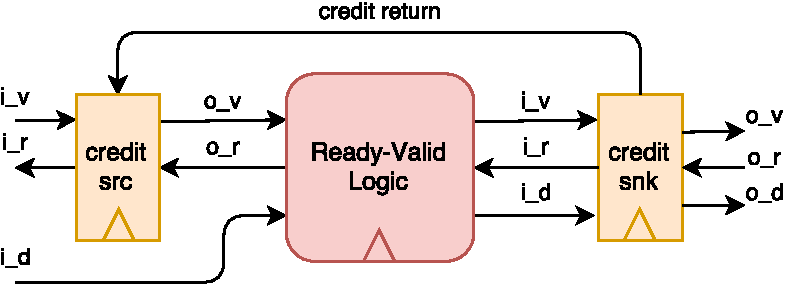
\includegraphics[width=0.70\textwidth]{7-credit.pdf}
  \caption{Diagram of a generalized transition between a credit- and ready-valid-based protocol.}
  \label{fig:7-credit}
\end{figure}



\subsection{Synchronization of Multiple Control Flows}
When designs get more complex, often multiple control flows have to be synchronized with each other before progress can be made. The cell library provides a single cell to synchronize \textit{N-to-M} inputs and outputs named \texttt{combine}. Two examples are shown below of uses of this cell during the implementation of the multi-stream buffer.



\subsubsection{Many-to-One}
\label{sec:sync-1}
The first encounter involves synchronization of multiple inputs with one output, as shown in \autoref{fig:7-sync-1}. In this example, the downstream module \textit{Request Consumer} is shared by two ready-valid-based modules, shown on the left of the \textit{Combine} cell. The \textit{Request Producer} produces a request consisting of a ready-valid pair and a stream identifier as associated data signal. Since a resource is shared downstream, that is only able to accept a predefined number of outstanding requests, each request from the producer has to obtain a unique tag.\\
There are various scenarios possible in this case. If the downstream module is not ready, both the \textit{Request Producer} and the \textit{Resource Manager} have to stall in order to prevent discarding a valid request or waste a precious tag, or both. Similarly, if the \textit{Request Producer} has no valid request, the \textit{Resource Manager} should not waste a tag and, vice versa, the \textit{Request Producer} should not discard a valid request when all tags are in use. The bottom line is that these two control flows have to synchronized.

\begin{figure}[H]
  \centering
  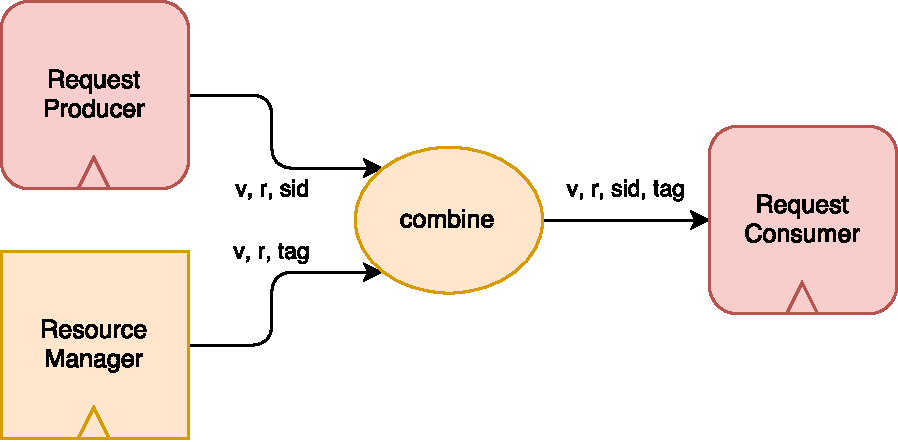
\includegraphics[width=0.70\textwidth]{7-sync-1.pdf}
  \caption{Diagram of a many-to-one synchronization example.}
  \label{fig:7-sync-1}
\end{figure}

To do so, the cell library provides a cell that can be configured to accommodate any number of inputs and outputs, independently of each other. \autoref{lst:sync-1} shows the ease of use of the \texttt{combine} cell (line 26), by simply connecting the various cells and modules together and configuring the number of inputs and outputs to synchronize. In this example, a hypothetical \textit{Request Producer} module is used and a simplified \textit{Resource Manager} cell from the library. The \texttt{res\_mgr} cell provides a configurable number of unique tags that can be used to associate with a request. The tag return interface has been omitted for simplicity.

\begin{lstlisting}[style={verilog-style}, caption=Many-to-One synchronization example., label=lst:sync-1]
  wire s1_req_v, s1_req_r;
  wire [nstrms_width-1:0] s1_req_sid;
  request_producer # (
    .width  (nstrms_width)
    ) is0_req_prod (
    .clk    (clk),
    .reset  (reset),
    .o_v    (s1_req_v),
    .o_r    (s1_req_r),
    .o_d    (s1_req_sid)
  );

  wire s1_mgr_v, s1_mgr_r;
  wire [tag_width-1:0] s1_mgr_tag;
  base_res_mgr # (
    .width  (tag_width)
    ) is1_res_mgr (
    .clk    (clk),
    .reset  (reset),
    .o_v    (s1_mgr_v),
    .o_r    (s1_mgr_r),
    .o_d    (s1_mgr_tag)
  );

  wire s1_comb_v, s1_comb_r;
  base_acombine # (
    .ni     (2),
    .no     (1)
    ) is1_cmb (
    .i_v    ({s1_req_v, s1_mgr_v}),
    .i_r    ({s1_req_r, s1_mgr_r}),
    .o_v    (s1_comb_v),
    .o_r    (s1_comb_r)
  );

  request_consumer # (
    .width  (nstrms_width),
    .tag    (tag_width)
    ) is2_req_cons (
    .clk    (clk),
    .reset  (reset),
    .i_v    (s1_comb_v),
    .i_r    (s1_comb_r),
    .i_sid  (s1_req_sid),
    .i_tag  (s1_mgr_tag)
  );
\end{lstlisting}



\subsubsection{One-to-Many}
Another encounter involves synchronization of a single input with multiple outputs, as shown in \autoref{fig:7-sync-2}. In this example, an incoming read request from the AFU starts two separate processes. The first process calculates an address to index a memory based on a global pointer stored in one of the \textit{Stream Pointer} modules and the number of other read ports accessing the same stream. The second process updates the global pointer based on all streams requested and will request new data upstream if needed. More details concerning the operation of the modules used can be found in Section \ref{sec:l1-ptr} and \ref{sec:rd-port}.\\
Similarly to the many-to-one synchronization example shown above, the \texttt{combine} cell is configured with the appropriate number of inputs and outputs and connects the incoming read request to both process modules. In essence, it would be similar to \autoref{lst:sync-1}, traversed in reverse order. While the two presented examples have either one input or output, the \texttt{combine} cell is able to synchronize any number of inputs with any number of outputs.

\begin{figure}[H]
  \centering
  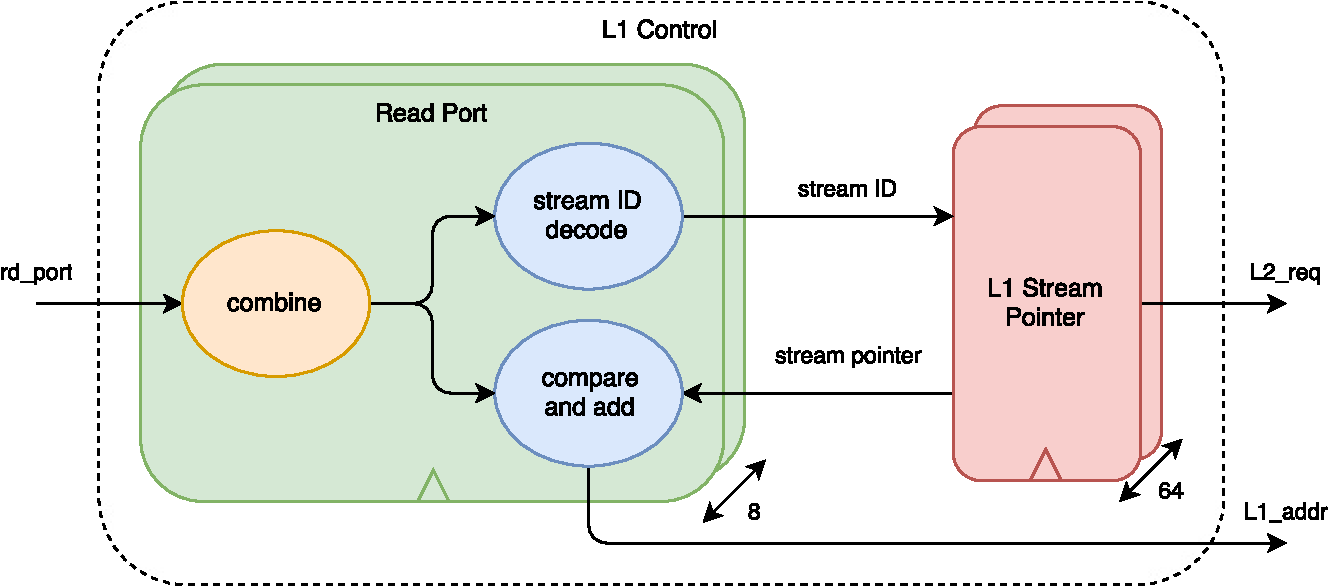
\includegraphics[width=0.90\textwidth]{7-sync-2.pdf}
  \caption{Diagram of a one-to-many synchronization example.}
  \label{fig:7-sync-2}
\end{figure}



\subsection{Timing Closure Using Relay Stations}
\label{sec:burp}
%\todo{
%- areg cell mostly used as reg and to fix timing. Other use cases for the base\_reg is when you have feedback in your path. You need a storage element otherwise it will be a combinatorial loop. A second use case is when you have converging paths to use this. Otherwise a deadlock will arise. These are advanced topics. If Andy would write a book it would be in advanced performance considerations.\\
%- Interesting topic is to prove if latch-burb is functionally equal to burb-latch. This can be set with the lbl parameter in the base\_reg module.
%}

The function of a relay station, as defined in the theory of latency-insensitive design \cite{delay-insensitive}, is fulfilled by the \texttt{reg} cell in the ready-valid design methodology. Typically the \texttt{reg} cell is used as a register for a ready-valid signal pair and the associated data signal. However, due to its parametrized nature, the cell can be easily reconfigured to meet timing by inserting an empty cycle, or to improve resource utilization by removing a cycle, either from the ready or valid path or both.\\
\autoref{lst:7-reg} shows the instantiation of the cell. It contains the typical ready-valid input and output signal pairs and a parameter \texttt{width} to configure the width of the data signal. Unique to this cell is the \texttt{lbl} parameter that stands for latch-burp-latch. When each bit is asserted, the respective cell (\texttt{latch} or \texttt{burp}) is generated.

\begin{lstlisting}[style={verilog-style}, caption=Ready-valid register cell from the ready-valid cell library., label=lst:7-reg]
base_areg # (
  .lbl    (3'b110),
  .width  (width)
) is0_reg (
  .clk    (clk),
  .reset  (reset),
  .i_v    (i_v),
  .i_r    (i_r),
  .i_d    (i_d),
  .o_v    (o_v),
  .o_r    (o_r),
  .o_d    (o_d)
);
\end{lstlisting}



\subsubsection{Latch Cell}
\autoref{lst:7-latch} shows the \texttt{latch} cell from the ready-valid cell library. This cell is used within the \texttt{reg} cell and provides a sequential element in the valid signal path. The \texttt{o\_v} signal is the output of a \texttt{vlat} cell of which the input signal is asserted only when the \texttt{latch} cell receives a valid input or when the downstream cell does not accept the current transfer. Similarly, when an associated data signal is present, an additional \texttt{vlat\_en} cell is generated and is only enabled if the downstream cell accepted the current transfer. This enable signal is also used to drive the \texttt{i\_r} signal.

\begin{lstlisting}[style={verilog-style}, caption=Latch cell from the ready-valid cell library., label=lst:7-latch]
module base_alatch #
(
  parameter width = 1
)
(
  input 	         clk,
  input 	         reset,
  input 	         i_v,
  input  [0:width-1] i_d,
  output 	         i_r,
  output 	         o_v,
  output [0:width-1] o_d,
  input 	         o_r
);

  wire o_v_in = i_v | (o_v & ~o_r);
  wire enable = o_r | ~o_v;
  assign i_r = o_r | ~o_v;
  base_vlat#(.width(1)) ivlat (.clk(clk), .reset(reset), .din(o_v_in), .q(o_v));

  wire [0:width-1] din = i_d[0:width-1];
  generate
    if (width > 0)
      base_vlat_en#(.width(width)) idlat (.clk(clk), .reset(1'b0), 
        .enable(enable), .din(i_d), .q(o_d));
  endgenerate

endmodule
\end{lstlisting}



\subsubsection{Burp Cell}
\autoref{lst:7-burp} shows the \texttt{burp} cell from the ready-valid cell library. This cell is used within the \texttt{reg} cell and provides a sequential element in the ready signal path. The \texttt{o\_v} signal propagates without any latency from the \texttt{i\_v} signal, unless the previous transfer was not completed, indicated by the \texttt{burp\_v} signal. Note that when \texttt{burp\_v} is asserted, the input data signal is not captured in the \texttt{vlat\_en} cell and the previously captured data signal is presented at the output. If not, the current input data is captured and presented and the output. The input ready signal is then equal to the inverse of the \texttt{burp\_v} signal.

\begin{lstlisting}[style={verilog-style}, caption=Burp cell from the ready-valid cell library., label=lst:7-burp]
module base_aburp #
(
  parameter width = 1
)
(
  input 	         clk,
  input 	         reset,
  input 	         i_v,
  input  [0:width-1] i_d,
  output 	         i_r,
  output 	         o_v,
  output [0:width-1] o_d,
  input 	         o_r
);

  wire burp_v;
  wire burp_v_in = ~o_r & (burp_v | i_v);
  assign i_r = ~burp_v;
  assign o_v = i_v | burp_v;
  base_vlat#(.width(1)) ivlat (.clk(clk), .reset(reset), .din(burp_v_in), .q(burp_v));
  
  generate
    if (width > 0) begin
      wire [0:width-1] burp_d;
      assign o_d = burp_v ? burp_d : i_d;
      base_vlat_en#(.width(width)) idlat (.clk(clk), .reset(1'b0), 
        .enable(~burp_v), .din(i_d), .q(burp_d));
    end
  endgenerate
endmodule
\end{lstlisting}





\subsubsection{Register Cell}
\autoref{fig:7-base-areg} shows a simplified view of the \texttt{reg} cell. Internally, the \texttt{burp} and \texttt{latch} cells, discussed in the previous paragraphs, are used. The orange ovals represent combinatorial logic, as shown in \autoref{lst:7-latch} and \autoref{lst:7-burp}.

\begin{figure}[H]
  \centering
  %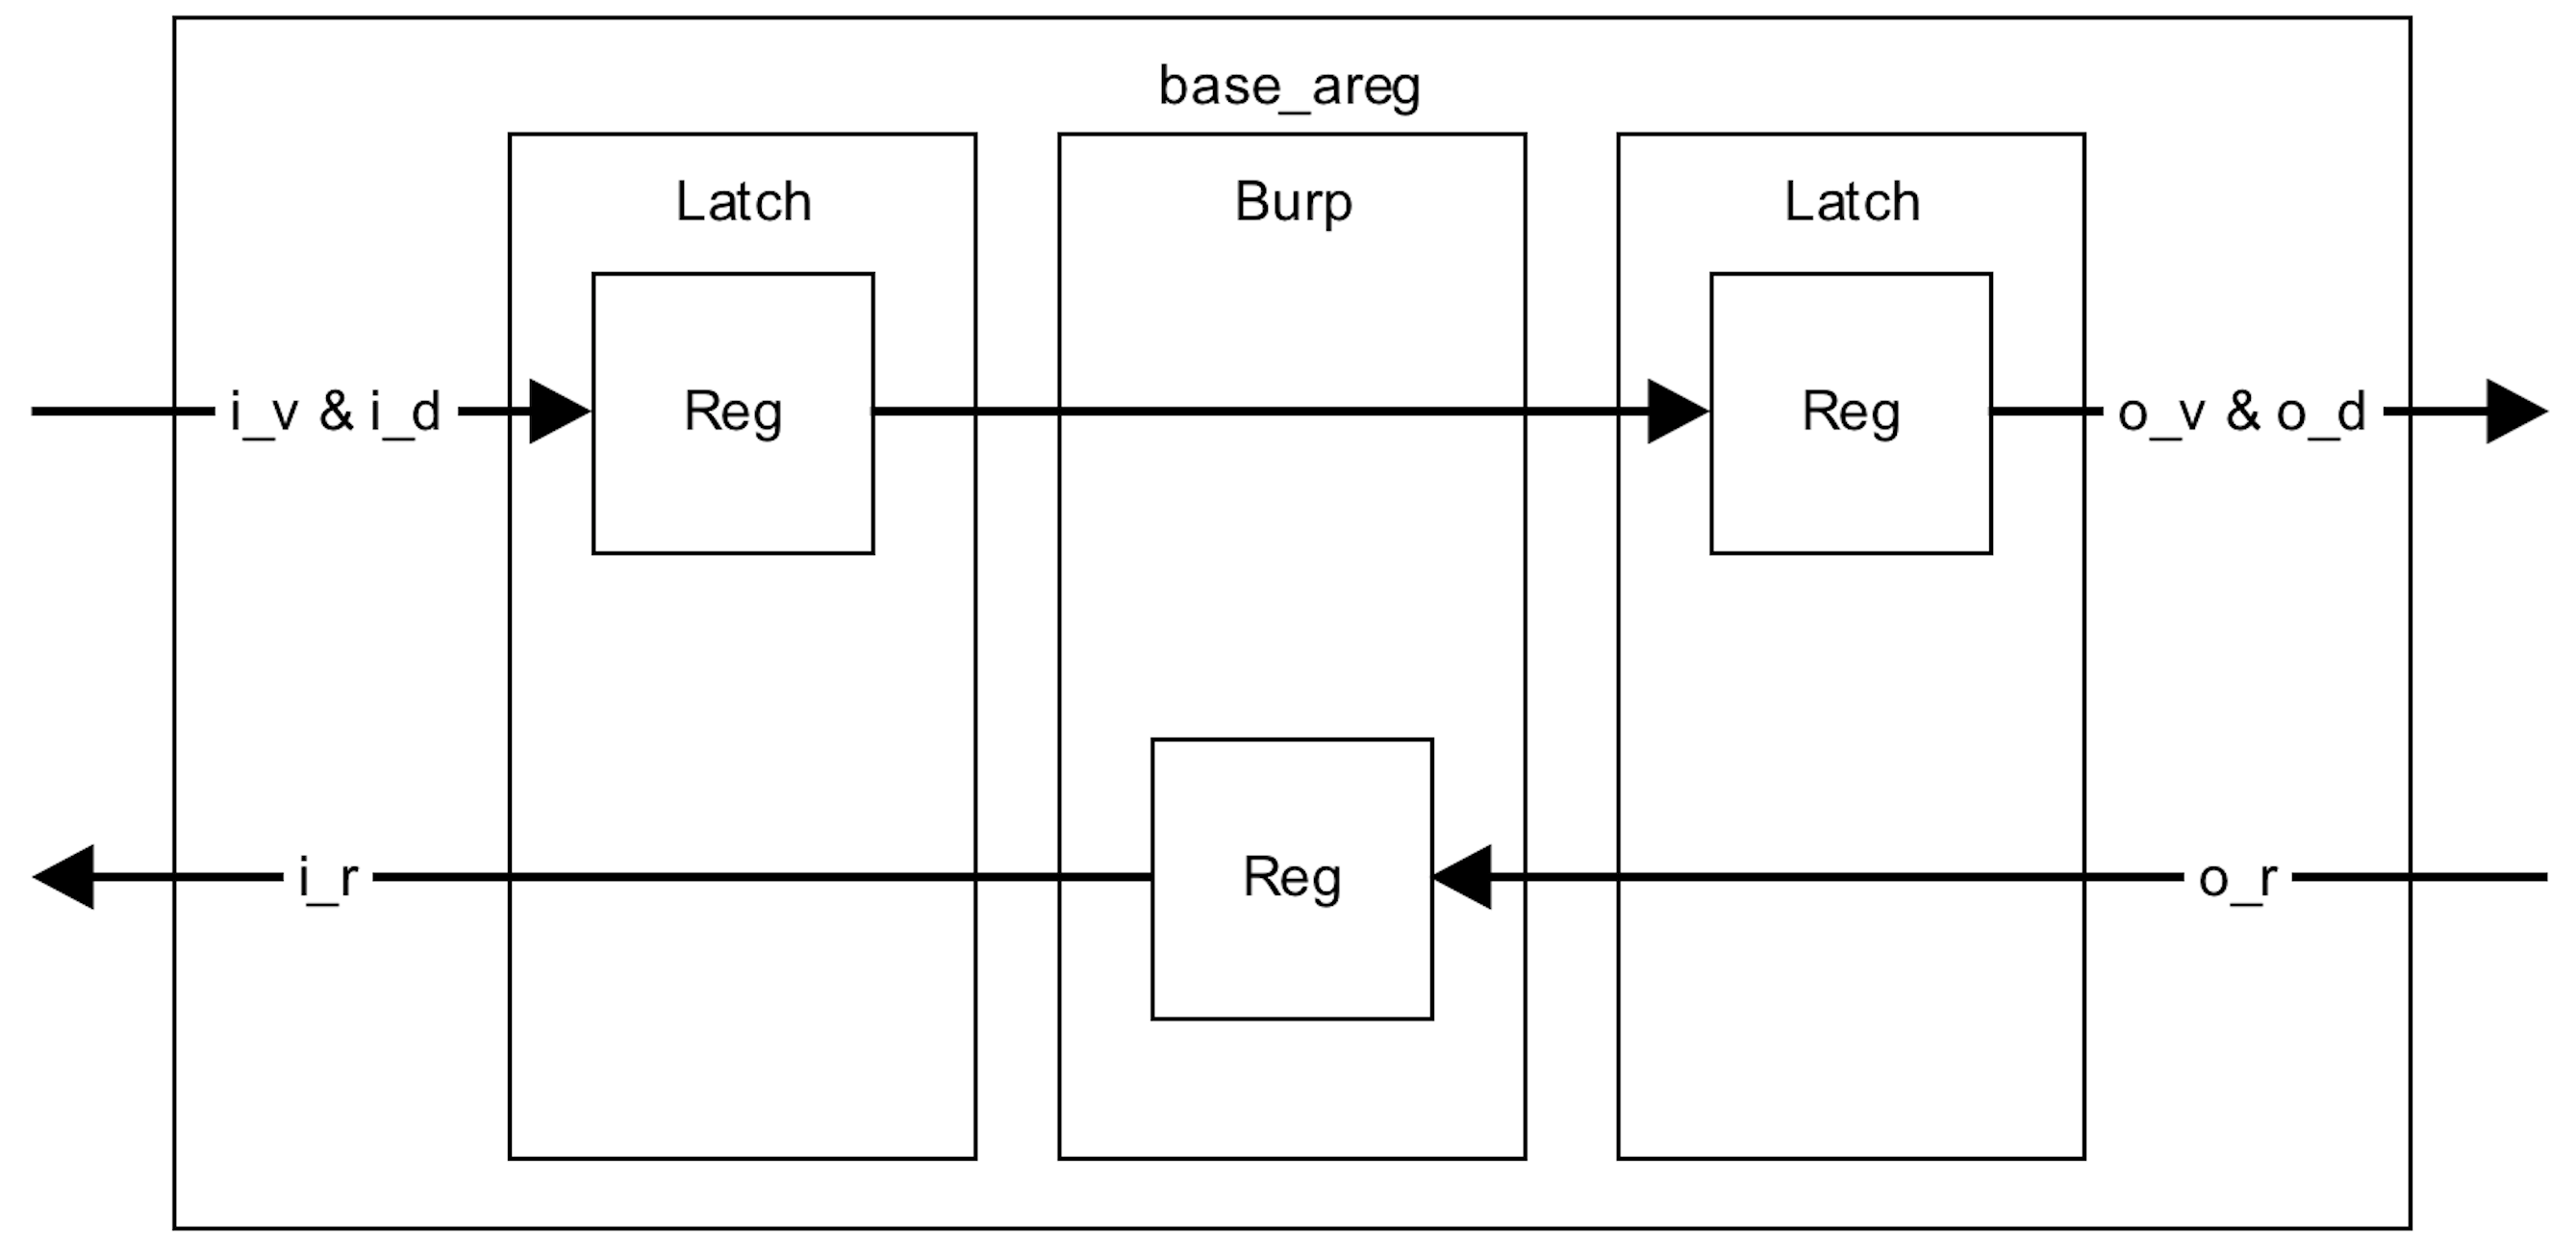
\includegraphics[width=0.75\textwidth]{7-base-areg.png}
  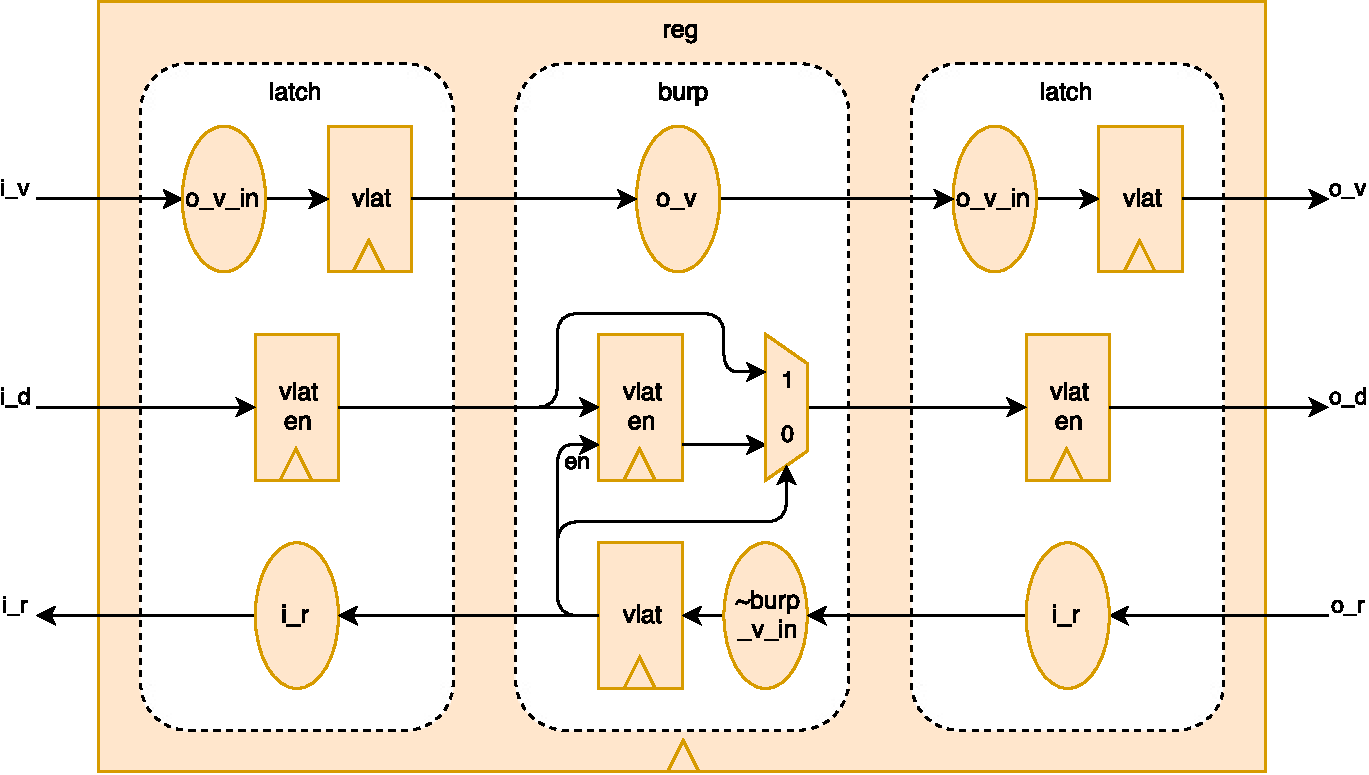
\includegraphics[width=0.75\textwidth]{6-reg.pdf}
  \caption[Diagram of the relay station cell with lbl - 3'b111.]{Diagram of the relay station cell with \texttt{lbl = 3'b111}.}
  \label{fig:7-base-areg}
\end{figure}

A typical starting point is to configure the cell as \texttt{3'b110} that generates one latch and one burp. This configuration is shown in \autoref{fig:7-base-areg-110} and results in a register in both the ready and valid paths. As mentioned in Section \ref{sec:workflow}, it is good practice to insert a \texttt{reg} cell regularly during the implementation to minimize rewriting of the system description at a later stage. By simply reconfiguring the relay station after the design failed timing, for example, a new compilation can be run immediately without rewriting any code.

\begin{figure}[H]
  \centering
  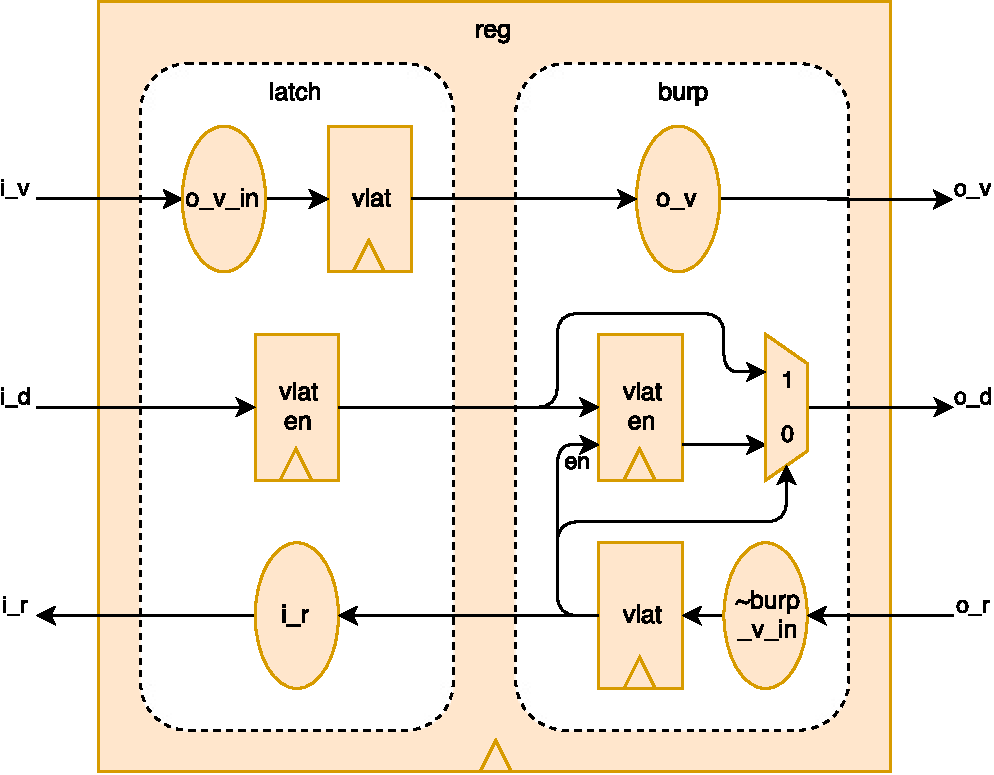
\includegraphics[width=0.50\textwidth]{6-reg-110.pdf}
  \caption[Diagram of the relay station cell with lbl = 3'b110.]{Diagram of the relay station cell with \texttt{lbl = 3'b110}.}
  \label{fig:7-base-areg-110}
\end{figure}
